\section{Asim e Asimtool}
Per la scrittura e la simulazione dei codici, saranno utilizzati i seguenti strumenti:
\begin{itemize}
    \item \textbf{ASIM}: Strumento per la simulazione del motorola 68k
    \item \textbf{ASIM-Tool}: Editor di testo e compilatore dei file .a68
\end{itemize}

\subsection{Asimtool}

Per asimtool, dopo aver scritto il file bisogna generare il file \.LIS, che poi sarà inserito all'interno del simultaore ASIM\. Tale file va generato secondo il seguente path: 
\\
\textbf{Assemble -> Assemble File <Nome\_File>.a68}
\\
Fatta tale operazione, nella cartella dove vi è salvato il file \.a68 dovrebbe essersi generato il file \.LIS
\\
Nel caso ci fossero particolari errori, asimtool li mostrerà a video specificando le righe su cui tali errori si presentano. Si invita a tenere ben cura della spaziatura tra i vari comandi e la loro leggittima posizione


\subsection{ASIM}
Una volta generato il file \.LIS con ASIM-tool, aprire ASIM ed impostare l'ambiente. Per impostare l'ambiente è richiesto un file cfg, che riporta i vari componenti che saranno mostrati all'interno del simulatore (tipo la memoria, il processore ecc.).
Il file base.cfg può essere trovato sui canali ufficiali degli studenti o può essere richiesto al professore. Tale file non contiene altro che una lista di componenti che verranno poi mostrati all'interno del simulatore.
Una volta aperto il file bisogna seguire il seguente path:
\\
\textbf{Window -> Tile}
\\
Tale opzione ci permette di poter vedere tutte le schermate aperte in maniera ordinata. Successivamente all'ordinamento delle schermate, bisogna "attivare" la configurazione, per fare ciò bisogna premere su di un tasto nella barra degli strumenti in Alto con illustrata una grossa I.
Una volta attivato il nostro ambiente, tenere cura di selezionare la finestra su cui c'è scritto di caricare il \.LIS. Una volta fatto questo in alto, tra i menu comparirà una nuova voce, ovvero: \textbf{Proc\_Unit}.
Una volta apparso tale menu basterà seguire il seguente path per poter selezionare il file \.LIS:
\\
\textbf{Proc\_Unit -> Load Assembler}
\\
Tale comando permetterà di poter caricare il file \.LIS generato da Asimtool, che dovrà essere selezionato appositamente tramite il file explorer.
Una volra caricato il file \.LIS bisognerà solo eseguire il programma.
Si consiglia, prima di eseguire, di attivare la visualizzazione dei registri interni. Tale cosa potrà essere fatta, selezionando la finestra in cui è caricato il file \.LIS e poi seguire il seguente path:
\\
\textbf{Proc\_Unit -> Show Registers}
\\
Questo permetterà di poter visualizzare i registri interni del processore nella parte bassa della finestra

\subsection{Esecuzione dei programmi}
Per l'esecuzione dei programmi, si può procedere in due modi:
\begin{itemize}
    \item \textbf{Passo Passo}: premendo sull'omino lento in alto
    \item \textbf{Fino alla fine}: premendo sull'omino che sembra correre
\end{itemize}

Il consiglio è sempre quello di verificare il funzionamento del programma passo passo e poi di utilizzare l'esecuzione veloce.

Per verificare o controllare particolari indirizzi di memoria si può utilizzare un tool interno.
Selezionando la memoria (quella che solitamente ha colori blu) e poi seguendo il seguente path:
\\
\textbf{Memory -> Show\_Loc}
\\
Si aprirà una finestra che ci permetterà di scrivere la locazione di memoria che vogliamo controllare. Una volta inserita e aver premuto "ok", la finestra mostrerà la memoria all'indirizzo richiesto in alto.

\subsection{Configurazione (file .cfg)} \label{par:cfg}

I sistemi hardware da simulare su ASIM sono caratterizzati da \textit{configurazioni}. Una configurazione contiene la descrizione degli oggetti da simulare e delle loro interconnesioni.
Gli oggetti simulabili da ASIM sono raggruppati in quattro categorie:

\begin{itemize}
    \item \textbf{Processore};
    \item \textbf{Nodo};
    \item \textbf{BUS/Memoria};
    \item \textbf{Device};
\end{itemize}

L'appartenenza di un oggetto ad una classe è determinata dal soddisfacimento di alcune proprietà.

\subsubsection{Processore}
\uppercase{è} un processore un qualsiasi dispositivo che ha lo stato interno rappresentato dal contenuto dei suoi registri più un insieme di informazioni riguardanti i bus a cui è connesso e un set di eventuali richieste di interruzioni.
Un processore gode delle seguenti proprietà:

\begin{itemize}
    \item Può eseguire un programma contenuto in memoria (interna al dispositivo o esterna);
    \item Può accedere attraverso il BUS ad una memoria esterna o ad altri dispositivi per operazioni di lettura o scrittura;
    \item Può servire e/o gestire interruzioni provenienti da altri dispositivi, eventualmente assegnando a questi un livello di priorità.
\end{itemize}

\subsubsection{Nodo}
\uppercase{è} un nodo un dispositivo che raccoglie informazioni relative alle connessioni con altri nodi ed ai messaggi in transito da/verso questi, e che gode delle seguenti proprietà:

\begin{itemize}
    \item può consentire la connessione tra dispositivi dello stesso tipo;
    \item può gestire, come nodo intermedio, la connessione tra dispositivi dello stesso tipo, instradando la comunicazione;
    \item può avere capacità autonome di elaborazione e trasformare i messaggi dati o ricevuti;
    \item Può essere connesso ad un BUS/memoria.
\end{itemize}

\subsubsection{BUS/Memoria}
\uppercase{è} dispositivo il cui stato interno è caratterizzato dai valori assunti da un insieme molto ampio di registri e/o da informazioni riguardanti i dispositivi  che esso connette e che gode delle seguenti proprietà:

\begin{itemize}
    \item può consentire a dispositivi di tipo processore di leggere o scrivere i suoi registri interni (la selezione avviene in base all'indirizzo);
    \item può consentire a dispositivi di tipo processore di leggere o scrivere i registri dei dispositivi di tipo device (la selezione avviene in base all'indirizzo);
    \item regola l'accesso di più dispositivi di tipo processore ai suoi registri ed ai device (in ogni istante al più un accesso è in corso, gli altri processori devono attendere);
    \item  gestisce la memoria fisica effettuando il “mapping” degli indirizzi virtuali negli indirizzi fisici;
    \item può consentire l'esecuzione di cicli non interrompibili di lettura-modifica;
    \item può connettersi ad altri dispositivi dello stesso tipo sia per costruire accessi da un altro bus sia verso un altro bus.
\end{itemize}

\subsubsection{Device}
\uppercase{è} un device tutto ciò che non rientra nelle categorie precedenti, e che gode delle seguenti proprietà:

\begin{itemize}
    \item può essere connesso ad un bus/memoria in modo che un processore possa accedere ad esso;
    \item può essere in grado di generare delle interruzioni da inviare ad un processore;
    \item  può essere connesso e comunicare con un altro device della stessa macchina o di un'altra macchina;
    \item può connettere dispositivi di tipo processore e bus/memoria a dispositivi del tipo bus/memoria.
\end{itemize}


\subsubsection{Generazione di configurazioni}
Dal menù \textit{edit} di ASIM è possibile generare una configurazione. I file che contengono le informazioni relative ad una configurazione hanno come estensione \textit{.cfg}.
La configurazione di un determinato oggetto viene specificata attraverso la compilazione manuale dei seguenti campi:

\begin{itemize}
    \item \textbf{Configuration Name}: Nome della configurazione corrente;
    \item \textbf{Chip Name}: Nome in codice dell'oggetto se esistono più oggetti in una classe;
    \item \textbf{Type}: Classe di appartenenza dell'oggetto;
    \item \textbf{Indentif}: Codice numerico che identifica il dispositivo nell'ambito della configurazione;
    \item \textbf{Bus}: Identificatore di un oggetto della classe Bus con cui lo specifico oggetto può interagire in qualche modo;
    \item \textbf{Address}: Indirizzi fisici compresi nello spazio di indirizzamento visto dall'oggetto;
    \item \textbf{com1,com2,...,com4}: Campi che codificano particolari caratteristiche dell'oggetto. 
\end{itemize}

Partiamo dalla configurazione di un oggetto di tipo \textbf{Processore}, esposta in figura \ref{img:cfg_CPU}:
\begin{figure}[htbp]
    \centering
    \fbox{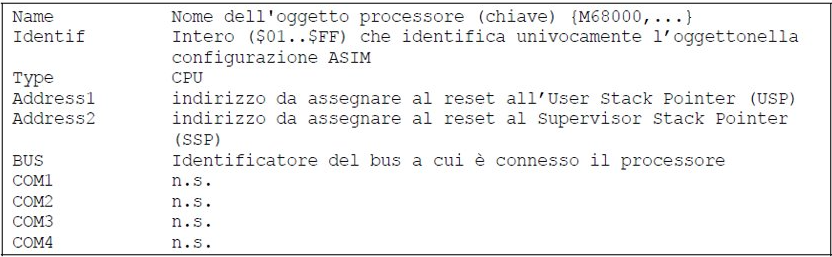
\includegraphics[width=0.8\textwidth]{img/cfg_CPU_1.png}}\\[0.5cm]
    \fbox{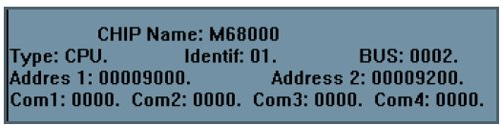
\includegraphics[width=0.6\textwidth]{img/cfg_CPU_2.png}}

    \caption{Configurazione CPU}
    \label{img:cfg_CPU}
\end{figure}

\uppercase{è} importante osservare che un generico device generante interruzioni può essere connesso ad un dispositivo in grado di gestirle (CPU, PIC). ASIM implementa un meccanismo di base di gestione delle interruzioni di tipo \textit{vettorizzato}: Tre linee, IPL0, IPL1, IPL2 (Interrupt request Priority Level) codificano l'evento interruzione in ingresso secondo il livello prioritario assegnato al dispositivo interrompente; Il processore, all'arrivo di un'interruzione (sia essa di tipo Hw che Sw) da servire (e non mascherare) avvia un ciclo di bus mediante il quale acquisisce dalla periferica interrompente uno specifico numero di vettore espresso su 8 bit (l'area ROM dei vettori occupa, infatti, il primo K dello spazio indirizzi di memoria); Tale numero, moltiplicato per 4 (mediante l'esecuzione di uno shift a sinistra di 2 posizioni), fornisce il puntatore ad una locazione di memoria ROM contenente il vettore associato all'Interrupt Service Routine (puntatore alla ISR).
Tutti i vettori sono di 32 bit (espressi su due word). Fa eccezione il vettore di reset numero 0, di 4 word di cui 2 usate per inizializzare il PC e 2 word per inizializzare il supervisor stack pointer.
Ogni segnale di interruzione è descritto da una struttura dati di 2 byte contenenti i seguenti tre campi:

\begin{itemize}
    \item \textbf{vector number}: bit b7-b0 del byte più significativo;
    \item \textbf{priority}: bit b7-b4 del byte meno significativo;
    \item \textbf{linea di interruzione}: bit b3-b0 del byte meno significativo.
\end{itemize}

Procediamo con la configurazione di un oggetto di tipo \textbf{Bus/Memoria}, esposta in figura \ref{img:cfg_MEM}:

\begin{figure}[htbp]
    \centering
    \fbox{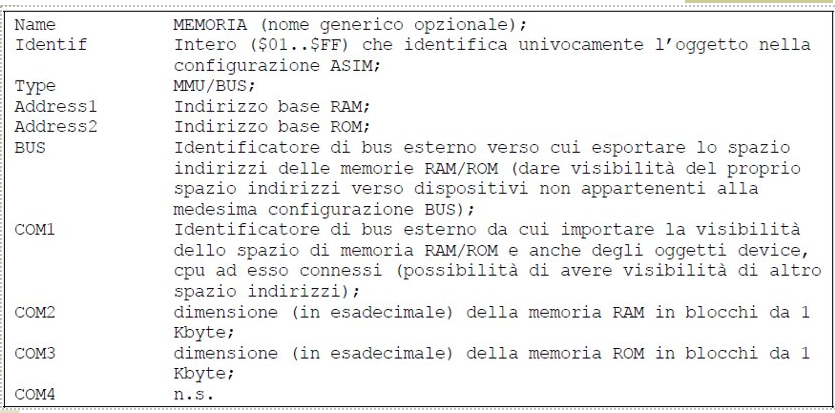
\includegraphics[width=1\textwidth]{img/cfg_bus_mem.png}}
    \caption{Configurazione BUS/Memoria}
    \label{img:cfg_MEM}
\end{figure}


\begin{figure}[htbp]
    \centering
    \fbox{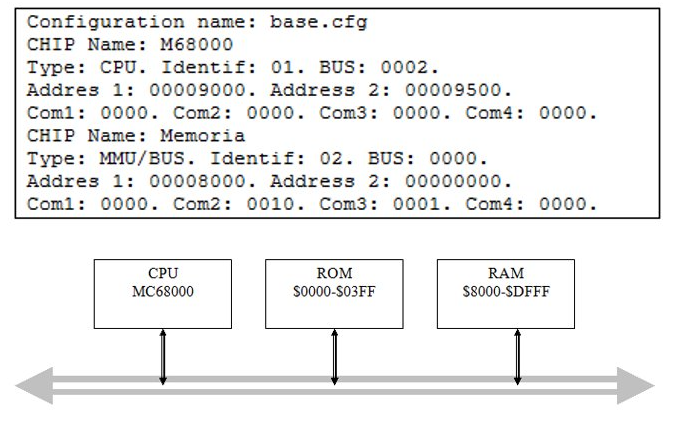
\includegraphics[width=.5\textwidth]{img/esempio_configurazione_1.png}}
    \caption{Esempio configurazione 1}
\end{figure}

\begin{figure}[htbp]
    \centering
    \fbox{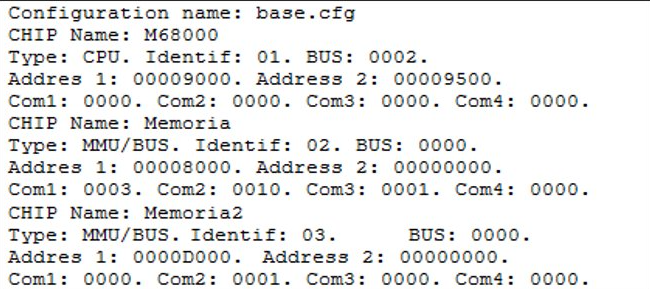
\includegraphics[width=0.77\textwidth]{img/esempio_cfg_2_1.png}}\\[0.5cm]
    \fbox{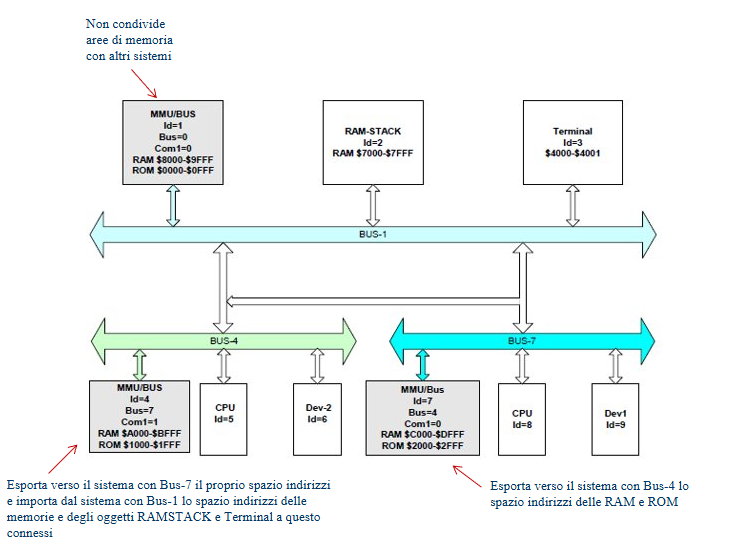
\includegraphics[width=0.77\textwidth]{img/esempio_cfg_2_2.png}}

    \caption{Esempio configurazione 2}
\end{figure}
